\section{Information Networks}

\subsection{Crawler Implementation}
\begin{lstlisting}[language=Python]
''' IMPORTS '''
# import HTML parser
from bs4 import BeautifulSoup

# import HTTP library
import requests

# import URL utility library
from urllib.parse import urlsplit

# import another URL utility library
import tldextract

# import sleep to prevent IP lockout
#     or intentional delays
from time import sleep

# import datetime to improve logging
from datetime import datetime

# python native queue data structure
from collections import deque

# native python json module, allows to serialize/deserialize json
import json
'''END IMPORTS'''

'''GLOBAL VARIABLES'''
# list of accepted domains
university_domains = ['uoit', 'ontariotechu'] 

# file extensions to be ignored
bad_file_extensions = ["mp4","mkv","pdf","docx","doc","mp3","wav","webp", "jpg", "png"]

# web page to begin traversing
INITIAL_URL = "https://ontariotechu.ca"

# this is a dictionary. each key is a URL and each value is a set of URLs that are referenced by the key
graph = {}

# this will be the queue of unvisited URLs
queue = deque()
'''END GLOBALS VARIABLES'''

''' BEGIN FUNCTIONS '''
# helper function to get formatted current datetime
def get_now():
    return datetime.now().strftime("%Y-%m-%d %H:%M:%S")

# lambda function to disregard all those hrefs that are not http or https pages
def filter_non_http(url):
    splitted_url = urlsplit(url)
    scheme = splitted_url.scheme
    if scheme not in ['http', 'https']:
        return False
    return True

# lambda function to filter off URLs with bad file extensions
def detect_bad_file_extensions(url):
    splitted_url = urlsplit(url)
    path = splitted_url.path

    for ext in bad_file_extensions:
        if ext in path:
            return False
    return True

# lambda function to 
def rstrip_url(url):
    splitted_url = urlsplit(url)
    scheme = splitted_url.scheme
    netloc = splitted_url.netloc
    path = splitted_url.path\
        .rstrip('/')\
        .replace('index.php', '')\
        .replace('index.html', '')\
        .replace('//','/')\
        .rstrip('/')
    new_url = f'{scheme}://{netloc}{path}'.rstrip('/')
    return new_url

# lambda function to convert uoit domain to ontariotechu
def uoit_to_ontariotechu(url):
    splitted_url = urlsplit(url)
    scheme = splitted_url.scheme
    netloc = splitted_url.netloc.replace('uoit','ontariotechu')
    path = splitted_url.path
    new_url = f'{scheme}://{netloc}{path}'.rstrip('/')
    return new_url

# key function for BFS. This expands the current node (URL)
def generate_children(url):
    try:
        # 1) sleep for 1 second to avoid ip blocking or slow down
        sleep(1)
        
        # 2) perform HTTP request to given URL
        print(get_now(), "GET HTTP request", url)
        r = requests.get(url)
        html_content = r.content

        # 3) parse HTML response to Python object
        soup = BeautifulSoup(html_content, "html.parser")

        # 4) get all anchor tags
        all_anchors = soup.find_all("a")
        
        # 5) get all hrefs from all anchors
        all_hrefs = []
        for anchor in all_anchors:
            try:
                all_hrefs.append(anchor['href'])
            except:
                pass

        # 6) filter off hrefs that are not in the UOIT or OTU domains
        university_hrefs = list(filter(lambda d: tldextract.extract(d).domain in university_domains, all_hrefs))

        # 7) filter off all URLs that are not http or https (e.g. mailto)
        university_hrefs = list(filter(filter_non_http, university_hrefs))

        # 8) filter off URLs that point to files
        university_hrefs = list(filter(detect_bad_file_extensions, university_hrefs))

        # 9) remove index.php or index.html, trailing slashes and double slashes
        university_hrefs = list(map(rstrip_url, university_hrefs))

        # 10) convert uoit domains to ontariotechu since uoit redirects to ontariotech
        university_hrefs = list(map(uoit_to_ontariotechu, university_hrefs))

        # 11) return all found children
        print(get_now(), 'Returning children...')
        return list(set(university_hrefs))
    except:
        return []

# bfs driver function
def bfs(url):
    print(get_now(), "Started BFS...")
    # 1) start by populating the queue with the initial node
    queue.append(url)

    # 2) while the queue isnt empty
    while len(queue) != 0:
        # 3) dequeue a node in a "first in first out" strategy
        u = queue.popleft()

        # 4) get current nodes of the graph
        graph_keys = list(graph.keys())

        # 5) if the popped item is not a node in the graph
        if u not in graph_keys:
            print(get_now(), f'Generating children of {u}...')
            # 6) expand all nodes from current node
            children = generate_children(u)
            print(get_now(), 'Generated', len(children), 'children!')

            # 7) append to queue all chosen links in current web page
            for child in children:
                queue.append(child)
            
            # 8) add current node's adjacency list
            graph[u]=children
        # 9) if web page has been visited before, skip
        else:
            print(get_now(), f'Skipped {u} !')

    # 10) after traversing all web pages, dump graph to a json file for posterior processing and analytics
    print(get_now(), 'Writing adjacency list to file...')
    with open('bfs_adj_list.json', 'w') as f:
        f.write(json.dumps(graph))
    print(get_now(), 'Wrote adjacency list to file!')

''' END FUNCTIONS '''


# Python's main function
''' BEGIN MAIN '''
if __name__ == '__main__':
    program_begin = datetime.now()
    print(program_begin, "Starting BFS...")
    # start BFS from initial URL
    bfs(INITIAL_URL)
    program_end = datetime.now()
    print(program_end, "Program finished!")
    delta = program_end - program_begin
    print("Program took", delta, "to complete!")
''' END MAIN '''
\end{lstlisting}

\subsection{Code Explanation}
\subsubsection{Imports}
BeautifulSoup is responsible for converting the HTML string retrieved from the website into a serialized Python object. This allows for easy querying of all HTML tags and their attributes.

The \textit{requests} library is used to perform HTTP GET requests. The actual web page information is stored in the response's \textit{content} property.

From \textit{urllib} I imported the urlsplit function to easily split the URL into scheme, domain, and path. Query string parameters were ignored. In the same line of though, \textit{tldextract} was also used to easily extract the domain of the URL and change it in a lambda function from \textit{uoit} to \textit{ontariotechu} if it was the case.

The \textit{sleep} function from module \textit{time} was imported to force a 2-second wait before issuing the next HTTP request. This was done to avoid throttling, which would slow down the crawler's activity, and to prevent the domain from locking out my IP.

The \textit{datetime} function from module \textit{datetime} was imported to simply print out current date and time. The reason behind this was to improve logging quality.

The \textit{deque} class was imported from module \textit{collections} to ease the development of the BFS algorithm. It is a queue data structure and allows for queueing and dequeueing elements in it. It works as the queue of web pages that have not been visited yet.

Finally, the \textit{json} module was imported to dump the assembled graph into a JSON file. Because the crawling was a time-consuming task, having the graph readily available is important.

\subsubsection{Global Variables}
A \textit{university\_domains} list containing \textit{uoit} and \textit{ontariotechu} was used to hold the two University's known domains. It is employed on the filtering of URLs that point to outside of the University's network. This way I can keep crawl only the pages that belong and refer to the Ontario Tech University.

The \textit{bad\_file\_extensions} list holds a few of the common file extensions that may be present on a URL. It, too, is used to filter off web pages that would host files. Since they are not actual web pages, it makes no sense to go through them.

Simply, the \textit{INITIAL\_URL} is just a variable that is used to trigger the Breadth First Search Algorithm. It is passed in the main method as the starting node.

The \textit{graph} variable is a dictionary that will be the assembled graph. The keys will be the URLs and the adjacency list will be a set of URLs the node has hyperlinks to.

Finally, the \textit{queue} variable starts as an empty queue. This queue is used to hold the web pages that have yet to be visited.

\subsubsection{Functions}
The \textit{get\_now} function is a wrapper for the \textit{datetime} function. It's only purpose is to return a formatted string containing the current date and time, for logging purposes.

Next, the \textit{filter\_non\_http} function is a lambda function. It is used in a \textit{filter} list function to remove all URLs that are not HTTP or HTTPS schemes. An example of a URL that was removed was a \textit{mailto}.

The \textit{detect\_bad\_file\_extensions} function is another lambda filter function. It works by splitting the URL and grabbing its path - the path is everything that comes after the country (e.g. \textit{.ca}) - and searching for any of the aforementioned bad file extensions.

Following the list of helper functions, the \textit{rstrip\_url} is another lambda function. This one, on the other hand, is used in a list mapping. It works by splitting a URL and altering the path to remove trailing slashes, any files that are index files (HTML or PHP). This function then returns the stripped URL.

The next lambda function is called \textit{uoit\_ontariotechu}. The sole purpose of this function is to map all URLs that are in the UOIT domain to Ontario Tech University's domain. This avoids adding nodes to the graph that are different in name, but that point to the same content.

Next, the core of the BFS algorithm, is the \textit{generate\_children} function. It works by trying to perform an HTTP GET request. When the request fails by any reason, I say that no children were found, since no web page was collected. If the request does not fail, I collect the content (namely, the HTML page as a string), parse it with \textit{BeautifulSoup}, query all anchor HTML tags, then try to collect every href attribute from the anchors. Next, I process all hrefs using a series of mappings and filters. I first filter off those URLs that are not in the UOIT/Ontario Tech University domain. Then the remaining URLs are filtered to remove every scheme that is not HTTP not HTTPS. The remaining URLs are again filtered to remove those that host files. Next, I map the URLs to remove trailing slashes and index pages. Finally, the remaining set of URLs is mapped again, but this time to change all UOIT domains into Ontario Tech University domains. After this series of mappings and filters, the remaining URLs are put into a set, which in Python removes duplicates from any list, and returned. This finishes the execution of the \textit{generate\_children} function.

Lastly, the \textit{bfs} function is the actual implementation of the Breadth First Search algorithm. It starts by pushing to the queue the URL that was passed as a parameter. Then, until the queue is not empty, it dequeues a node that has not been visited yet and gets the current list of nodes in the graph. If the dequeued node is not in the list of nodes, expand the graph by generating the current node's children. Then, for each child of the current node, add it to the queue then add all children as the adjacency list of the current node in the graph. if the dequeued node is in the list of nodes in the graph, skip it to avoid performing unnecessary HTTP requests. When the queue is empty, the function dumps the assembled graph to a JSON file for persistent storage and avoid running the crawler every time the graph is needed.

\subsubsection{Main}
The main function in Python is used to call the \textit{bfs} function. It passes the \textit{INITIAL\_URL} as parameter. This function is the starting point of a Python program. It also calculates how long it took for the crawler to finish traversing all web pages in the Ontario Tech University's domain.

\subsection{Analyses}
After dumping the graph to a JSON file, the contents were read as a string and converted back to a dictionary. Using NetworkX, this dictionary was then used to instantiate a directed graph. All metrics were extracted using NetworkX.

\subsubsection{Directed or undirected?} The network formed by the web pages within the University's domain is a directed graph. This choice is due to the fact that even though web page A has a hyperlink to web page B, there is no guarantee that web page B will have a hyperlink to web page A. Also, when traversing a graph in a search, it is not interesting to be able to go back to the previous node. This risks the search never finding a solution.

\subsubsection{Weighted or unweighted?} This graph was modelled to have unweighted edges. The reason for this is that the objective was to only traverse the web pages within the University's domain. Therefore, the main interest was to know whether or not one web page has a hyperlink to another. However, even if it is desired to find the most referenced node, one can accomplish this by querying the graph for the node with the greatest in-degree.

\subsubsection{Metrics}
\textbf{Number of nodes.} The total number of nodes, that is, unique web pages within the University's domain is \textbf{2916}.

\textbf{Number of edges.} The total number of edges, that is, how many hyperlinks exist within the University's domain is \textbf{109213}.

\textbf{Edge density.} Defined in equation \ref{equation:undir_density}, the density for the graph formed by the University's web pages is \textbf{0.0128}.

\textbf{Degree distribution.} Figure \ref{fig:6} shows the degree distribution for this network's graph. Figure \ref{fig:otu_deg_dist} shows the degree distribution in normal scale. Figure \ref{otu_deg_dist_log_log} shows the degree distribution in log scale. Doing log-log scaling allows us to better see what the degree distribution looks like. The first figure may indicate that the degree distribution for this graph follows a power law. This would mean that a great number of nodes have low degree, meaning that web page does not reference may pages, and few pages refer it back.

\begin{figure}
    \centering
    \subfloat[\centering Degree distribution]{{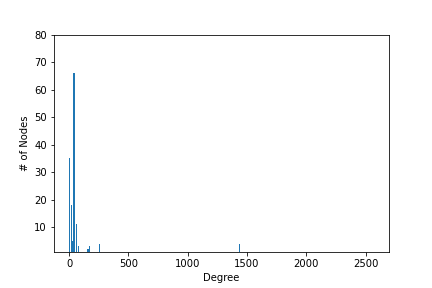
\includegraphics[width=0.45\textwidth]{img/otu_degree_distribution.png}\label{fig:otu_deg_dist}}}
    \qquad
    \subfloat[\centering Degree distribution (log-log)]{{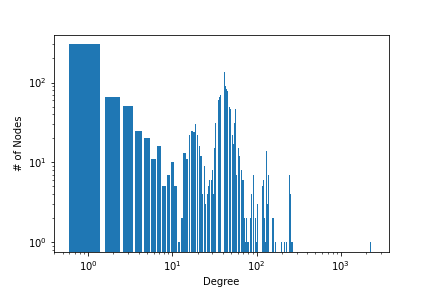
\includegraphics[width=0.45\textwidth]{img/otu_log_log_degree_distribution.png}\label{otu_deg_dist_log_log}}}
    \caption{Degree distributions}
    \label{fig:6}
\end{figure}

\textbf{Average clustering coefficient.} Previously defined in equation \ref{equation:avg_clustering_coef}, the average clustering coefficient for the graph assembled by traversing all web pages in the University's domain is \textbf{0.456}.

\textbf{Number of nodes in strongly connected component.} The number of nodes in the subgraph detected by querying the strongly connected component is \textbf{2225}.

\textbf{Number of nodes in weakly connected component.} The number of nodes in the subgraph detected by querying the weakly connected component is \textbf{2916}.

\textbf{Average path length in SCC.} For the strongly connected component of the graph, the average path length is \textbf{4.685}.

\textbf{Average path length in WCC.} The average path length of the weakly connected component is \textbf{3.710}.

\textbf{Diameter in SCC.} The diameter of the strongly connected component is \textbf{64}.

\textbf{Diameter in WCC.} For the weakly connected component, however, NetworkX's implementation calculates is to be infinite because the directed graph is not strongly connected. Therefore, I calculated the diameter as though the graph is undirected. The diameter in this case becomes \textbf{8}.

\textbf{Community detection.}